\chapter{Resultados} \label{ch:Resultados}

En este capítulo se mostrarán todas las figuras\footnote{Para todas las simulaciones $\mu=1$. 
Las dimensiones de este parámetro y de $\lambda$ son de $tiempo^{-1}$. Se utilizará un sistema de unidades arbitrario,
lo que quiere decir que se producirá una recuperación por hora, día, mes... Debido a esta arbitrariedad en las unidades,
hemos decidido omitirlas en todas las gráficas. Además, la condición inicial para todos los casos 
exceptuando la sección \ref{sec:ccii}, la condición inicial es que el número de infectados inicial es $N/10$}
obtenidas a partir de las simulaciones. Se estudiará la evolución del número de infectados frente al tiempo,
cómo afectan las condiciones iniciales, el número medio de infectados frente a la tasa de infección y el cambio de 
la desviación estándar de diferentes tamaños de población.

\section{Series temporales}
En las figuras \ref{f:n vs t Gillespie 1000} y \ref{f:n vs t Focker 1000} se muestra cómo evoluciona el número de infectados frente al 
tiempo para diferentes tasas de infección $\lambda$ en una población de $N=1000$ individuos. Encontraremos un estado transitorio en el que se produce 
la infección o recuperación de la población de la población en función de la tasa de infección y pasado este tiempo, se llega al estado 
estacionario, donde el número de infectados oscilará en torno al valor estacionario obtenido en la ecuación \ref{eq:ecuación de langevin}.

\begin{figure}[H]
    \begin{center}
      \begin{subfigure}
          [Gillespie.]{
          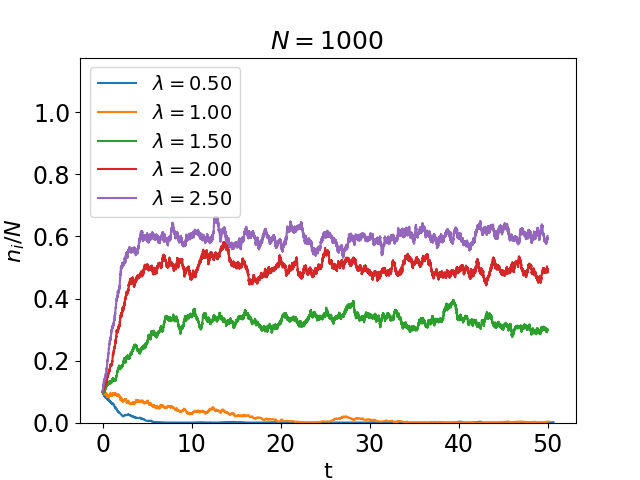
\includegraphics[width=0.5\textwidth]{ni_t_1000.png}
          \label{f:n vs t Gillespie 1000}}
      \end{subfigure}
  
      \vspace{0.5cm}
      
      \begin{subfigure}
          [Langevin.]{
          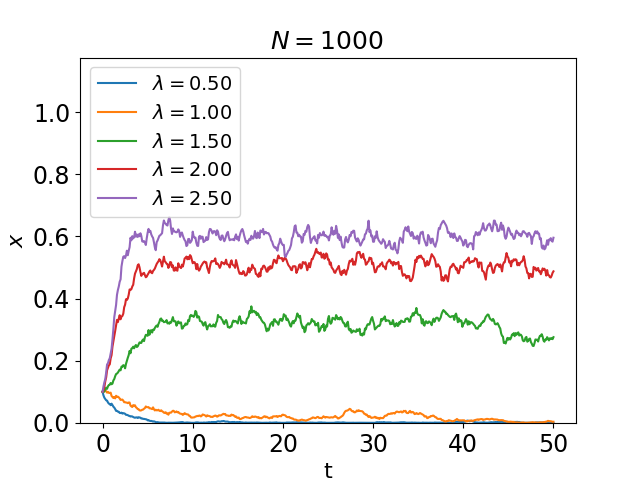
\includegraphics[width=0.5\textwidth]{x vs t fockerplanck.png}
          \label{f:n vs t Focker 1000}}
      \end{subfigure}
      
      \caption{Número de infectados frente al tiempo para una población de 1000 individuos.}
      \label{f:n vs t 1000}
    \end{center}    
\end{figure}
  

Como se puede comprobar, encontramos un período transitorio hasta que llegamos al estado estacionario, en el que para el caso en el que 
$\mu > \lambda$ el número de infectados tiende a cero, ya que hay mayor probabilidad de recuperación que de infección. Por otro lado, cuando
$\mu < \lambda$ el número de infectados oscilará en torno al valor estacionario que hemos obtenido en la ecuación \ref{eq: xest}.
\newpage
Podemos analizar también cómo cambian las fluctuaciones para poblaciones más grandes. Aumentando en un orden de magnitud la población, las 
fluctuaciones se reducirán en un factor $1/\sqrt{N}$ tal y como aparece en la ecuación de Langevin \ref{eq:ecuación de langevin}. En las figuras  
\ref{f:n vs t Gillespie 10000} y \ref{f:n vs t Focker 10000} podemos ver la atenuación de estas fluctuaciones. En general, todas las trayectorias
para poblaciones mayores serán similares, pero con fluctuaciones más pequeñas, por lo que no es necesario conocer el estado estacionario 
dichas poblaciones. Debido a que el tiempo de simulación aumenta con el $N$ en la resolución con el algoritmo de Gillespie, 
nos restringiremos a poblaciones de $10$, $100$ y $1000$ individuos. 

\begin{figure}[H]
    \begin{center}
      \begin{subfigure}
          [Gillespie.]{
          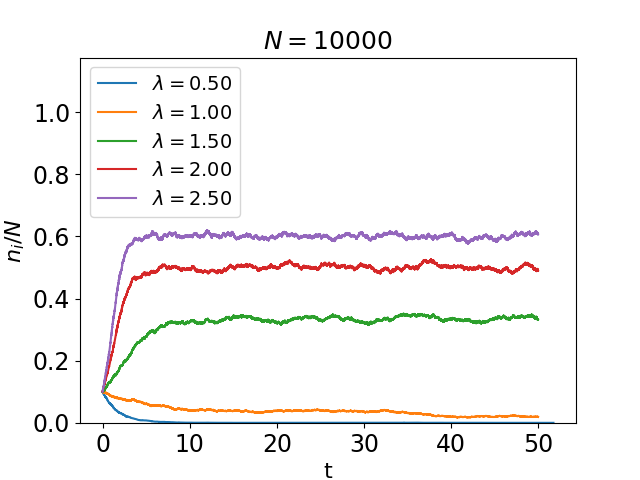
\includegraphics[width=0.5\textwidth]{ni_t_10000.png}
          \label{f:n vs t Gillespie 10000}}
      \end{subfigure}
  
      \vspace{0.5cm}
      
      \begin{subfigure}
          [Langevin.]{
          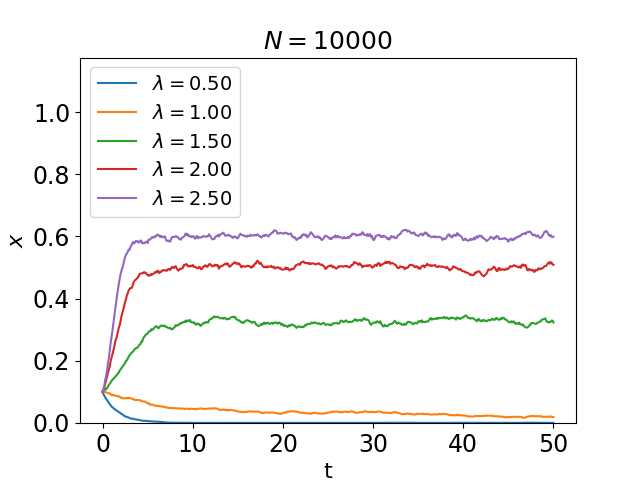
\includegraphics[width=0.5\textwidth]{x vs t fockerplanck 10000.png}
          \label{f:n vs t Focker 10000}}
      \end{subfigure}
      
      \caption{Número de infectados frente al tiempo para una población de 10000 individuos.}
      \label{f:n vs t 10000}
    \end{center}    
\end{figure}


\section{Efecto de las condiciones iniciales}\label{sec:ccii}

A continuación, veremos cómo el estado estacionario es independiente al número de infectados inicial, al estar
tratando con procesos de Markov, los cuales solo dependen del estado del sistema en el tiempo anterior. Además, esto también
queda explícito en la ecuación de Langevin \ref{eq:ecuación de langevin}, donde no aparece ningún término referido a las condiciones iniciales.
Se muestran en la figura \ref{f:ccii} la evolución del número de infectados frente al tiempo para diferentes condiciones iniciales.



\begin{figure}[H]
    \begin{center}
      \begin{subfigure}
          [Gillespie.]{
          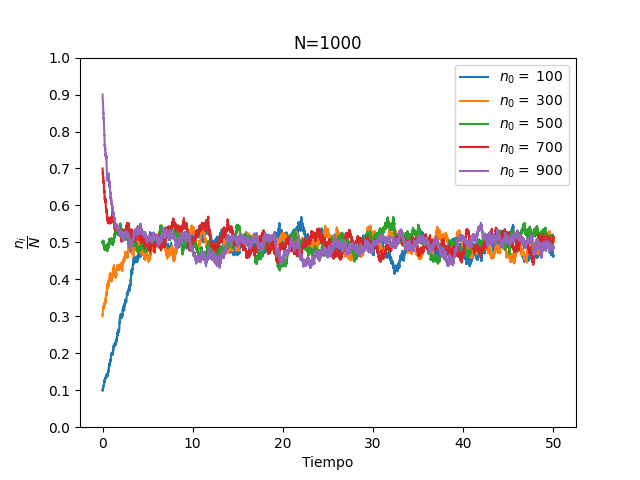
\includegraphics[width=0.5\textwidth]{Ccii.png}
          \label{f:gillespie ccii}}
      \end{subfigure}
  
      \vspace{0.5cm}
      
      \begin{subfigure}
          [Langevin.]{
          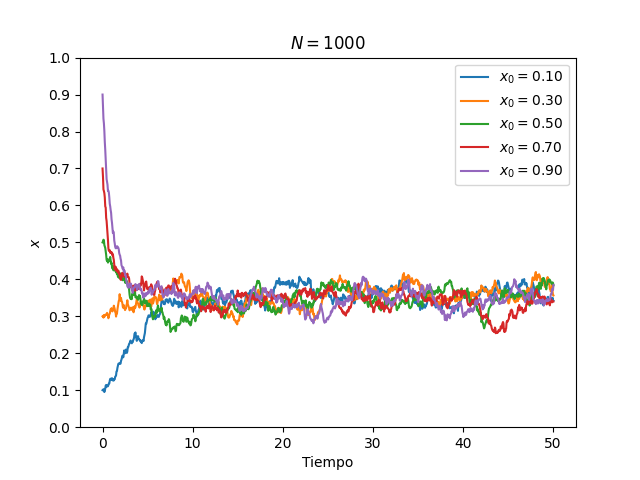
\includegraphics[width=0.5\textwidth]{cciifockerplanck.png}
          \label{f:focker ccii}}
      \end{subfigure}
      
      \caption{Número de infectados frente al tiempo para diferentes condiciones iniciales.}
      \label{f:ccii}
    \end{center}    
\end{figure}

Como vemos, usando tanto el algoritmo de Gillespie como la solución de la ecuación de Langevin se obtiene el mismo comportamiento llegando a un 
mismo estado estacionario, que se corresponde con el valor dado de la ecuación \ref{eq: xest}. En este caso, las tasas de infección y recuperación
son $\lambda=2$ y $\mu=1$.
\newpage
\section{Diagrama de fase}

En este apartado estudiaremos el número medio de infectados frente a la tasa de infección, obteniendo así curvas
similares a la de la figura \ref{f:diagrama modelo sis}. En las figuras \ref{f:gillespie diagrama fase} y \ref{f:focker diagrama fase}
se encuentran dichas curvas.


\begin{figure}[H]
    \begin{center}
      \begin{subfigure}
          [Gillespie.]{
          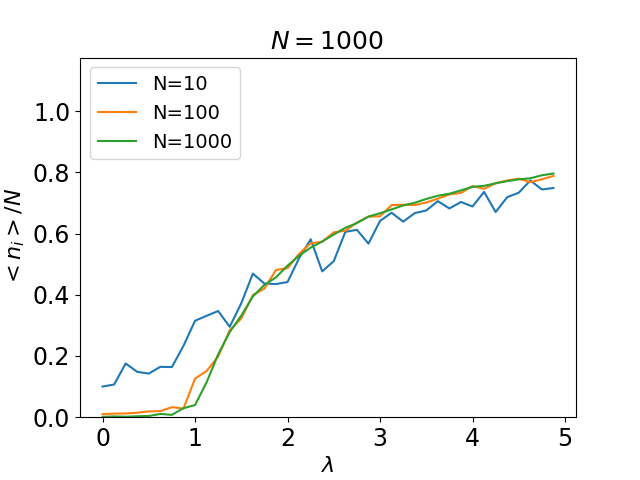
\includegraphics[width=0.5\textwidth]{40 puntos 10_100_1000.png}
          \label{f:gillespie diagrama fase}}
      \end{subfigure}
  
      \vspace{0.5cm}
      
      \begin{subfigure}
          [Langevin.]{
          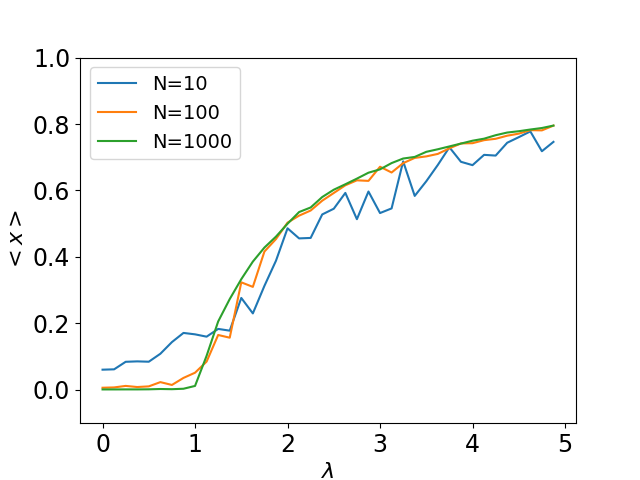
\includegraphics[width=0.5\textwidth]{xmedia vs lambda focker.png}
          \label{f:focker diagrama fase}}
      \end{subfigure}
      
      \caption{Número medio de infectados frente a la tasa de infección para distintas poblaciones.}
      \label{f:diagrama de fase}  
    \end{center}    
\end{figure}



Como se puede comprobar, ambas figuras se ajustan bastante bien a lo esperado, si bien en el caso en el que la población es de $10$ individuos
esta curva es levemente distinta, ya que el cambio de estado de un individuo cambia el $10\%$ del sistema. A esto tenemos que 
sumarle que nuestra condición inicial para esta población es que un individuo está infectado, por lo que las propias fluctuaciones llevan 
a la extinción de infectados y nuestra simulación añade uno infectado para seguir ejecutándose, lo que provoca que el número medio de infectados
sea no nulo en la zona absorbente.

\section{Desviación estandar}

Es importante estudiar el comportamiento de las fluctuaciones a lo largo del diagrama de fase, ya que estas en el entorno del punto crítico 
podrán cambiar el sistema de la zona absorbente a la activa. A continuación, en la figura \ref{f:diagrama de fase desviación} se muestra el
diagrama de fase para la desviación estándar.

\begin{figure}[H]
    \begin{center}
      \begin{subfigure}
          [Gillespie.]{
          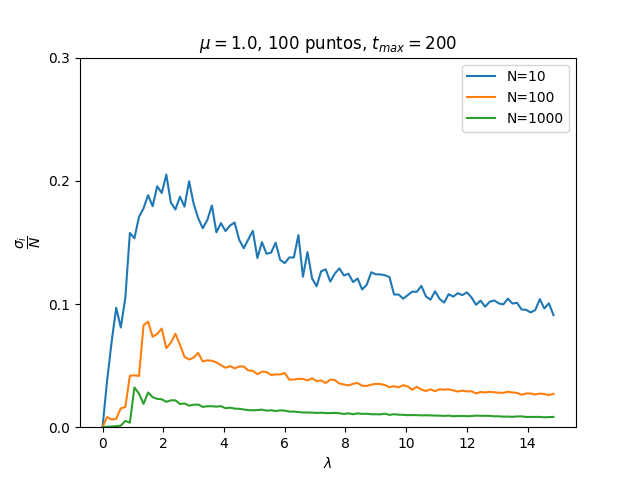
\includegraphics[width=0.5\textwidth]{sigma_lambda.png}
          \label{f:gillespie diagrama fase desviacion}}
      \end{subfigure}
  
      \vspace{0.5cm}
      
      \begin{subfigure}
          [Langevin.]{
          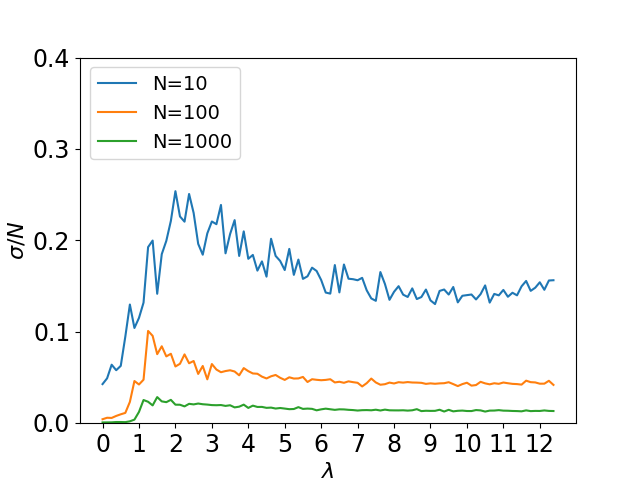
\includegraphics[width=0.5\textwidth]{sigmalambdafocker.png}
          \label{f:focker diagrama dase desviacion}}
      \end{subfigure}
      
      \caption{Desviación estándar frente a la tasa de infección para diferentes poblaciones.}
      \label{f:diagrama de fase desviación}  
    \end{center}    
\end{figure}


Como se comprueba en las figuras, tanto el algoritmo de Gillespie como la resolución de la ecuación de Langevin proporcionan un 
comportamiento similar. Estas fluctuaciones son mayores en el entorno del punto crítico, tal y como se ha comentado 
en la sección \ref{sec:modelo sis}, ya que es donde los proesos estocásticas toman mayor importancia. Por otro lado, se puede 
comprobar que en el caso de la solución de la ecuación de Langevin para diez individuos tenemos una pequeña sobreestimación de
la desviación estándar, pues para obtener esta, hemos supuesto la aproximación de grandes tamaños para llegar a la ecuación 
de Fokker-Planck y en este caso, la aproximación no es correcta. Podemos utilizar esta desviación estándar como las barras de error,
pero hemos decidido no incluirlas en el diagrama de fase para no sobrecargar la imagen.
